Peningkatan margin keselamatan yang telah dibahas pada
Subbab~\ref{sec:analisis_keselamatan} berpotensi memengaruhi efisiensi
navigasi, karena robot yang mempertahankan jarak lebih jauh dari
\textit{obstacle} cenderung memilih lintasan yang lebih konservatif, baik
melalui penyesuaian arah maupun pengurangan kecepatan. Subbab ini
mengevaluasi konsekuensi tersebut melalui tiga metrik efisiensi yang telah
didefinisikan pada Subbab~\ref{sec:metrik}: waktu navigasi
(Persamaan~\ref{eq:avg_vel} terkait), panjang lintasan
(Persamaan~\ref{eq:path_length}), dan rata-rata kecepatan linear
(Persamaan~\ref{eq:avg_vel}), untuk menjawab apakah peningkatan keselamatan
yang diperoleh metode usulan harus dibayar dengan penurunan efisiensi
navigasi yang berarti. Penilaian terhadap besar-kecilnya konsekuensi ini
disampaikan setelah seluruh analisis deskriptif dan statistik berikut
dipaparkan secara lengkap.

\begin{table}[H]
\centering
\caption{Persentase perubahan metrik efisiensi dan keselamatan pada
konfigurasi \textit{proposed method} relatif terhadap \textit{baseline}.}
\label{tab:tradeoff_persen}
\resizebox{\textwidth}{!}{%
\begin{tabular}{lcccc}
\toprule
\textbf{Pasangan} & \textbf{$\Delta$ Waktu (\%)} & \textbf{$\Delta$ Lintasan (\%)} & \textbf{$\Delta$ Kec. Linear (\%)} & \textbf{$\Delta$ Clearance (\%)} \\
\midrule
S1--S5 & +21,6 & -0,1 & -17,7 & n/a \\
S2--S6 & +15,5 & -0,7 & -14,1 & +1,6 \\
S3--S7 & +63,7 & +5,9 & -35,0 & +198,4 \\
S4--S8 & +40,1 & +4,1 & -23,5 & +2164,3$^{*}$ \\
\bottomrule
\end{tabular}%
}
\vspace{1mm}

{\footnotesize $^{*}$Lihat catatan pada Tabel~\ref{tab:clearance_deskriptif},
Subbab~\ref{sec:analisis_keselamatan}, mengenai persentase yang tidak stabil
akibat \textit{baseline} mendekati nol.}
\end{table}

\begin{figure}[H]
\centering
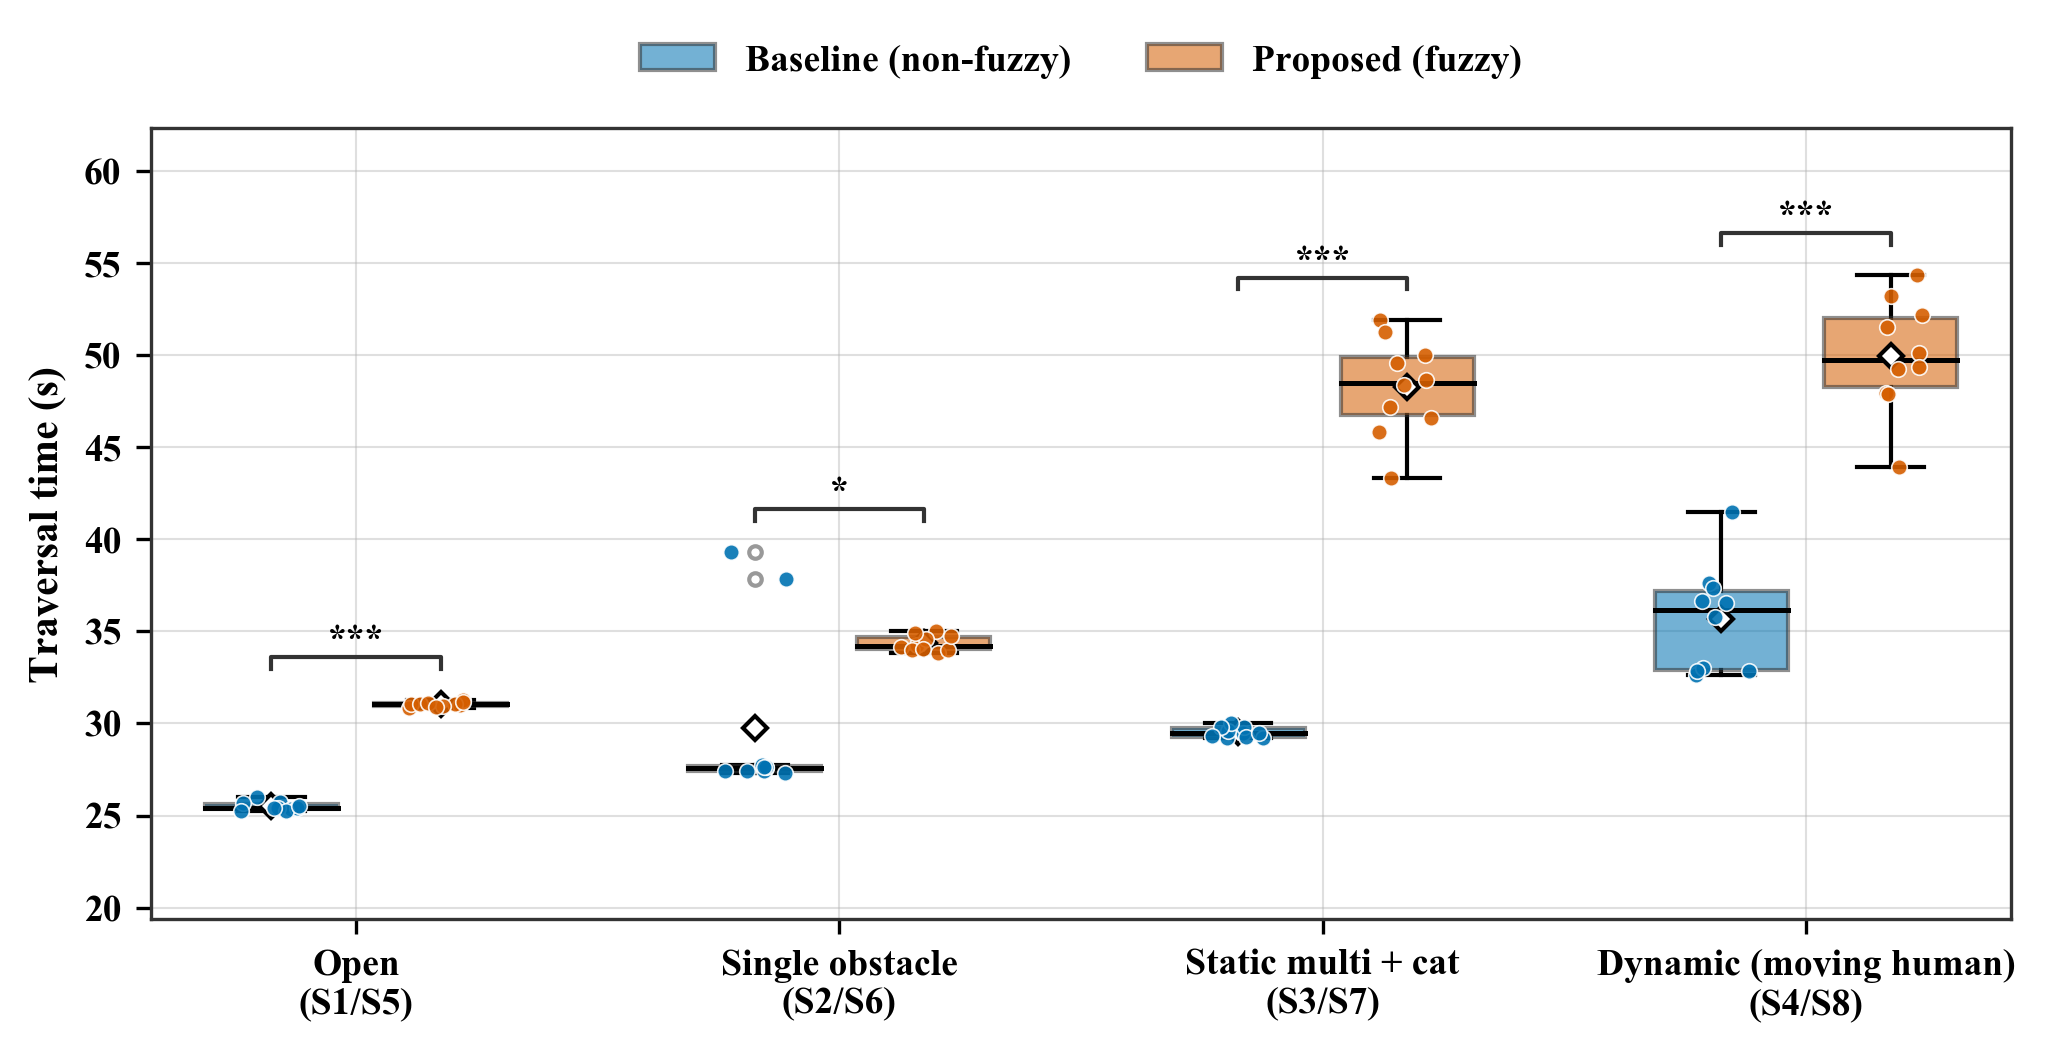
\includegraphics[width=0.85\textwidth]{gambar/4.5_tradeoff_scatter.png}
\caption{Hubungan antara minimum clearance (sumbu-x) dan waktu tempuh
(sumbu-y) untuk seluruh 80 \textit{trial}. Warna menandakan konfigurasi
(\textit{baseline}/\textit{proposed}), bentuk marker menandakan lingkungan
pengujian.}
\label{fig:tradeoff_scatter}
\end{figure}

Tabel~\ref{tab:tradeoff_persen} dan Gambar~\ref{fig:tradeoff_scatter}
menunjukkan bahwa konfigurasi \textit{proposed method} secara umum
membutuhkan waktu tempuh yang lebih lama dibandingkan \textit{baseline}
pada seluruh pasangan skenario, dengan peningkatan berkisar antara
+15,5\% (S2/S6) hingga +63,7\% (S3/S7). Peningkatan waktu tempuh paling
besar konsisten ditemukan pada pasangan yang melibatkan \textit{obstacle}
bersuhu rendah pada area \textit{blind-spot} (S3/S7) dan \textit{obstacle}
dinamis (S4/S8), yaitu kondisi yang juga menunjukkan peningkatan minimum
clearance paling besar pada Subbab~\ref{sec:analisis_keselamatan}.

Berbeda dengan waktu tempuh, perubahan panjang lintasan relatif kecil pada
seluruh pasangan, berkisar antara $-0,7\%$ hingga $+5,9\%$. Pada S1/S5 dan
S2/S6, panjang lintasan \textit{proposed method} bahkan sedikit lebih
pendek dibandingkan \textit{baseline} ($-0,1\%$ dan $-0,7\%$), sementara
pada S3/S7 dan S4/S8 terdapat sedikit peningkatan ($+5,9\%$ dan $+4,1\%$).
Perubahan pada keempat pasangan ini tergolong kecil dan tidak
mengindikasikan bahwa robot menempuh rute yang jauh berbeda secara
geometris.

Pada metrik kecepatan linear, konfigurasi \textit{proposed method} secara
konsisten menghasilkan nilai rata-rata yang lebih rendah dibandingkan
\textit{baseline} pada seluruh pasangan skenario, dengan penurunan berkisar
antara $-14,1\%$ hingga $-35,0\%$. Pola ini konsisten dengan perilaku
navigasi yang lebih berhati-hati, mengingat pengurangan kecepatan adaptif
merupakan salah satu mekanisme adaptasi fuzzy yang telah dijelaskan pada
Subbab~\ref{sec:fuzzy_mamdani}.

Perbedaan ketiga metrik efisiensi antara kedua konfigurasi diuji
menggunakan uji Mann-Whitney U, dengan hipotesis yang sama seperti pada
Subbab~\ref{sec:analisis_keselamatan}:
\begin{itemize}
    \item $H_0$: tidak terdapat perbedaan distribusi metrik antara
    konfigurasi \textit{baseline} dan \textit{proposed method}.
    \item $H_1$: terdapat perbedaan distribusi metrik antara kedua
    konfigurasi (uji dua arah).
\end{itemize}

\begin{table}[H]
\centering
\caption{Hasil uji Mann-Whitney U untuk metrik efisiensi pada keempat
pasangan skenario ($\alpha=0,05$).}
\label{tab:tradeoff_mwu}
\begin{tabular}{llccc}
\toprule
\textbf{Metrik} & \textbf{Pasangan} & \textbf{$U$} & \textbf{$p$} & \textbf{Signifikan} \\
\midrule
\multirow{4}{*}{Waktu Tempuh (s)}
 & S1--S5 & 0  & 0,0002 & *** \\
 & S2--S6 & 20 & 0,0257 & *  \\
 & S3--S7 & 0  & 0,0002 & *** \\
 & S4--S8 & 0  & 0,0002 & *** \\
\midrule
\multirow{4}{*}{Panjang Lintasan (m)}
 & S1--S5 & 79 & 0,0243 & *  \\
 & S2--S6 & 20 & 0,0254 & *  \\
 & S3--S7 & 0  & 0,0002 & *** \\
 & S4--S8 & 4  & 0,0006 & *** \\
\midrule
\multirow{4}{*}{Kecepatan Linear (m/s)}
 & S1--S5 & 100 & 0,0002 & *** \\
 & S2--S6 & 80  & 0,0251 & *  \\
 & S3--S7 & 100 & 0,0002 & *** \\
 & S4--S8 & 99  & 0,0002 & *** \\
\bottomrule
\end{tabular}
\end{table}

Tabel~\ref{tab:tradeoff_mwu} menunjukkan bahwa seluruh dua belas kombinasi
pasangan-metrik signifikan secara statistik pada $\alpha=0,05$, dengan
tingkat signifikansi bervariasi dari cukup signifikan ($p<0,05$) pada
beberapa kombinasi di S2/S6 hingga sangat signifikan ($p<0,001$) pada
sebagian besar kombinasi lainnya.

\begin{table}[H]
\centering
\caption{Effect size (\textit{rank-biserial correlation}) untuk metrik
efisiensi pada keempat pasangan skenario.}
\label{tab:tradeoff_effect_size}
\begin{tabular}{llcc}
\toprule
\textbf{Metrik} & \textbf{Pasangan} & \textbf{Effect Size ($r$)} & \textbf{Interpretasi} \\
\midrule
\multirow{4}{*}{Waktu Tempuh}
 & S1--S5 & +1,00 & Besar \\
 & S2--S6 & +0,60 & Besar \\
 & S3--S7 & +1,00 & Besar \\
 & S4--S8 & +1,00 & Besar \\
\midrule
\multirow{4}{*}{Panjang Lintasan}
 & S1--S5 & -0,58 & Besar \\
 & S2--S6 & +0,60 & Besar \\
 & S3--S7 & +1,00 & Besar \\
 & S4--S8 & +0,92 & Besar \\
\midrule
\multirow{4}{*}{Kecepatan Linear}
 & S1--S5 & -1,00 & Besar \\
 & S2--S6 & -0,60 & Besar \\
 & S3--S7 & -1,00 & Besar \\
 & S4--S8 & -0,99 & Besar \\
\bottomrule
\end{tabular}
\end{table}

Tabel~\ref{tab:tradeoff_effect_size} menunjukkan bahwa seluruh dua belas
kombinasi tergolong effect size besar ($|r| \geq 0,50$) berdasarkan kriteria
pada Tabel~\ref{tab:effect_size}. Meskipun demikian, signifikansi statistik
dan effect size yang besar tidak selalu berarti perbedaan tersebut bermakna
secara praktis. Pada pasangan S1/S5, panjang lintasan menunjukkan effect
size besar ($r=-0,58$) meskipun selisih absolutnya hanya 0,01~m ($-0,1\%$),
karena variansi panjang lintasan pada kedua kelompok memang sangat kecil
sehingga selisih sekecil itu pun konsisten terdeteksi oleh uji
\textit{rank-based}. Sebaliknya, pada waktu tempuh S3/S7, effect size besar
($r=+1,00$) disertai selisih absolut yang juga besar ($+63,7\%$), sehingga
pada kombinasi ini signifikansi statistik dan kepentingan praktis sejalan.
Perbandingan ini menegaskan pentingnya membaca effect size bersama selisih
absolut pada Tabel~\ref{tab:tradeoff_persen}, bukan effect size semata.

Secara umum, peningkatan minimum clearance yang diperoleh metode usulan
disertai konsekuensi berupa waktu tempuh yang lebih lama dan kecepatan
linear yang lebih rendah, sementara panjang lintasan relatif tidak berubah.
Konsekuensi waktu tempuh paling besar muncul pada skenario yang paling
kompleks (S3/S7 dan S4/S8), yang juga merupakan skenario dengan peningkatan
keselamatan paling besar, mengindikasikan bahwa \textit{trade-off} ini
cenderung muncul justru ketika manfaat keselamatannya paling dibutuhkan.
Namun, \textit{trade-off} ini tidak seragam dan tidak selalu besar: pada
S2/S6, peningkatan waktu tempuh ($+15,5\%$) terjadi meskipun peningkatan
clearance sangat kecil ($+1,6\%$), menunjukkan bahwa hubungan antara
keselamatan dan efisiensi tidak selalu proporsional pada seluruh kondisi
lingkungan.

Tujuan utama penelitian ini adalah meningkatkan keselamatan navigasi pada
kondisi \textit{blind-spot} dan lingkungan dinamis, sehingga penurunan
efisiensi dalam batas yang dijelaskan di atas dapat dipandang sebagai
konsekuensi yang dapat diterima apabila disertai peningkatan margin
keselamatan yang sepadan, sebagaimana ditunjukkan pada S3/S7 dan S4/S8.
Meskipun demikian, dapat diterima atau tidaknya \textit{trade-off} ini pada
akhirnya bergantung pada kebutuhan aplikasi spesifik; pada aplikasi yang
sangat mengutamakan kecepatan operasional, peningkatan waktu tempuh sebesar
40--64\% pada skenario kompleks tetap perlu dipertimbangkan secara cermat.
Penelitian ini tidak mengklaim bahwa metode usulan unggul secara mutlak,
melainkan menawarkan satu titik keseimbangan tertentu antara keselamatan
dan efisiensi.

Beberapa keterbatasan perlu dicatat dalam membaca hasil ini. Pertama,
besaran \textit{trade-off} yang teramati dapat dipengaruhi oleh parameter
\textit{tuning} fuzzy dan APF yang digunakan pada penelitian ini
(Subbab~\ref{sec:fuzzy_mamdani}), sehingga konfigurasi parameter yang
berbeda dapat menghasilkan titik keseimbangan keselamatan-efisiensi yang
berbeda. Kedua, simulator Gazebo tidak sepenuhnya merepresentasikan
dinamika dunia nyata, termasuk gesekan permukaan dan keterlambatan aktuator
yang dapat memengaruhi waktu tempuh aktual. Ketiga, jumlah \textit{trial}
yang terbatas ($n=10$ per skenario) membatasi presisi estimasi besaran
\textit{trade-off} ini.

Selain efisiensi global yang telah dibahas di atas, kualitas gerakan robot
selama navigasi juga perlu dievaluasi. Subbab berikutnya membahas aspek
kehalusan gerak dan osilasi melalui metrik kecepatan angular, disajikan
pada Subbab 4.6.